\documentclass[twoside]{book}

% Packages required by doxygen
\usepackage{fixltx2e}
\usepackage{calc}
\usepackage{doxygen}
\usepackage[export]{adjustbox} % also loads graphicx
\usepackage{graphicx}
\usepackage[utf8]{inputenc}
\usepackage{makeidx}
\usepackage{multicol}
\usepackage{multirow}
\PassOptionsToPackage{warn}{textcomp}
\usepackage{textcomp}
\usepackage[nointegrals]{wasysym}
\usepackage[table]{xcolor}

% Font selection
\usepackage[T1]{fontenc}
\usepackage[scaled=.90]{helvet}
\usepackage{courier}
\usepackage{amssymb}
\usepackage{sectsty}
\renewcommand{\familydefault}{\sfdefault}
\allsectionsfont{%
  \fontseries{bc}\selectfont%
  \color{darkgray}%
}
\renewcommand{\DoxyLabelFont}{%
  \fontseries{bc}\selectfont%
  \color{darkgray}%
}
\newcommand{\+}{\discretionary{\mbox{\scriptsize$\hookleftarrow$}}{}{}}

% Page & text layout
\usepackage{geometry}
\geometry{%
  a4paper,%
  top=2.5cm,%
  bottom=2.5cm,%
  left=2.5cm,%
  right=2.5cm%
}
\tolerance=750
\hfuzz=15pt
\hbadness=750
\setlength{\emergencystretch}{15pt}
\setlength{\parindent}{0cm}
\setlength{\parskip}{3ex plus 2ex minus 2ex}
\makeatletter
\renewcommand{\paragraph}{%
  \@startsection{paragraph}{4}{0ex}{-1.0ex}{1.0ex}{%
    \normalfont\normalsize\bfseries\SS@parafont%
  }%
}
\renewcommand{\subparagraph}{%
  \@startsection{subparagraph}{5}{0ex}{-1.0ex}{1.0ex}{%
    \normalfont\normalsize\bfseries\SS@subparafont%
  }%
}
\makeatother

% Headers & footers
\usepackage{fancyhdr}
\pagestyle{fancyplain}
\fancyhead[LE]{\fancyplain{}{\bfseries\thepage}}
\fancyhead[CE]{\fancyplain{}{}}
\fancyhead[RE]{\fancyplain{}{\bfseries\leftmark}}
\fancyhead[LO]{\fancyplain{}{\bfseries\rightmark}}
\fancyhead[CO]{\fancyplain{}{}}
\fancyhead[RO]{\fancyplain{}{\bfseries\thepage}}
\fancyfoot[LE]{\fancyplain{}{}}
\fancyfoot[CE]{\fancyplain{}{}}
\fancyfoot[RE]{\fancyplain{}{\bfseries\scriptsize Generated by Doxygen }}
\fancyfoot[LO]{\fancyplain{}{\bfseries\scriptsize Generated by Doxygen }}
\fancyfoot[CO]{\fancyplain{}{}}
\fancyfoot[RO]{\fancyplain{}{}}
\renewcommand{\footrulewidth}{0.4pt}
\renewcommand{\chaptermark}[1]{%
  \markboth{#1}{}%
}
\renewcommand{\sectionmark}[1]{%
  \markright{\thesection\ #1}%
}

% Indices & bibliography
\usepackage{natbib}
\usepackage[titles]{tocloft}
\setcounter{tocdepth}{3}
\setcounter{secnumdepth}{5}
\makeindex

% Hyperlinks (required, but should be loaded last)
\usepackage{ifpdf}
\ifpdf
  \usepackage[pdftex,pagebackref=true]{hyperref}
\else
  \usepackage[ps2pdf,pagebackref=true]{hyperref}
\fi
\hypersetup{%
  colorlinks=true,%
  linkcolor=blue,%
  citecolor=blue,%
  unicode%
}

% Custom commands
\newcommand{\clearemptydoublepage}{%
  \newpage{\pagestyle{empty}\cleardoublepage}%
}

\usepackage{caption}
\captionsetup{labelsep=space,justification=centering,font={bf},singlelinecheck=off,skip=4pt,position=top}

%===== C O N T E N T S =====

\begin{document}

% Titlepage & ToC
\hypersetup{pageanchor=false,
             bookmarksnumbered=true,
             pdfencoding=unicode
            }
\pagenumbering{alph}
\begin{titlepage}
\vspace*{7cm}
\begin{center}%
{\Large Transport controller for Miranda }\\
\vspace*{1cm}
{\large Generated by Doxygen 1.8.13}\\
\end{center}
\end{titlepage}
\clearemptydoublepage
\pagenumbering{roman}
\tableofcontents
\clearemptydoublepage
\pagenumbering{arabic}
\hypersetup{pageanchor=true}

%--- Begin generated contents ---
\chapter{Module Index}
\section{Modules}
Here is a list of all modules\+:\begin{DoxyCompactList}
\item \contentsline{section}{Transport Controller}{\pageref{group__transport__controller}}{}
\begin{DoxyCompactList}
\item \contentsline{section}{Feed Forward Controller}{\pageref{group__group__feed__forward}}{}
\item \contentsline{section}{Robot Arm Controller}{\pageref{group__group__arm__controller}}{}
\end{DoxyCompactList}
\end{DoxyCompactList}

\chapter{Hierarchical Index}
\section{Class Hierarchy}
This inheritance list is sorted roughly, but not completely, alphabetically\+:\begin{DoxyCompactList}
\item \contentsline{section}{Orientation\+Feed\+Forward}{\pageref{classOrientationFeedForward}}{}
\begin{DoxyCompactList}
\item \contentsline{section}{Ros\+Orientation\+Feed\+Forward$<$ T $>$}{\pageref{classRosOrientationFeedForward}}{}
\end{DoxyCompactList}
\end{DoxyCompactList}

\chapter{Class Index}
\section{Class List}
Here are the classes, structs, unions and interfaces with brief descriptions\+:\begin{DoxyCompactList}
\item\contentsline{section}{\hyperlink{classConstrainedrigid__motion}{Constrainedrigid\+\_\+motion} }{\pageref{classConstrainedrigid__motion}}{}
\item\contentsline{section}{\hyperlink{classConstrainedrigid__motionRos}{Constrainedrigid\+\_\+motion\+Ros} }{\pageref{classConstrainedrigid__motionRos}}{}
\item\contentsline{section}{\hyperlink{classConstrainedrigid__motionTf}{Constrainedrigid\+\_\+motion\+Tf} }{\pageref{classConstrainedrigid__motionTf}}{}
\item\contentsline{section}{\hyperlink{classController}{Controller} }{\pageref{classController}}{}
\item\contentsline{section}{\hyperlink{structController_1_1ControlVector}{Controller\+::\+Control\+Vector} \\*Defines the controllers output }{\pageref{structController_1_1ControlVector}}{}
\item\contentsline{section}{\hyperlink{classInputAllocException}{Input\+Alloc\+Exception} }{\pageref{classInputAllocException}}{}
\item\contentsline{section}{\hyperlink{classInputBase}{Input\+Base} }{\pageref{classInputBase}}{}
\item\contentsline{section}{\hyperlink{classInputOdom}{Input\+Odom} }{\pageref{classInputOdom}}{}
\item\contentsline{section}{\hyperlink{classInputPoseOdom}{Input\+Pose\+Odom} }{\pageref{classInputPoseOdom}}{}
\item\contentsline{section}{\hyperlink{classInputPoseTwist}{Input\+Pose\+Twist} }{\pageref{classInputPoseTwist}}{}
\item\contentsline{section}{\hyperlink{classLyapunovController}{Lyapunov\+Controller} }{\pageref{classLyapunovController}}{}
\item\contentsline{section}{\hyperlink{structLyapunovController_1_1LyapunovParameter}{Lyapunov\+Controller\+::\+Lyapunov\+Parameter} \\*Holds the necessary parameters for the control law }{\pageref{structLyapunovController_1_1LyapunovParameter}}{}
\item\contentsline{section}{\hyperlink{classMsgOrientationFeedForward}{Msg\+Orientation\+Feed\+Forward$<$ T $>$} \\*A Ros implementation of the Orientation\+Feeed\+Forward class. It contains a ros Subscriber that listens to a specific message and uses the message data as input data for the feed forward control }{\pageref{classMsgOrientationFeedForward}}{}
\item\contentsline{section}{\hyperlink{classNecessaryParamException}{Necessary\+Param\+Exception} }{\pageref{classNecessaryParamException}}{}
\item\contentsline{section}{\hyperlink{classOrientationFeedForward}{Orientation\+Feed\+Forward} \\*A Orientation feed forward class. It uses a given orientation and calculates a robot arm pose that compansates the motion by the change of orientation (null space motion) }{\pageref{classOrientationFeedForward}}{}
\item\contentsline{section}{\hyperlink{classPassTroughController}{Pass\+Trough\+Controller} }{\pageref{classPassTroughController}}{}
\item\contentsline{section}{\hyperlink{classRosOrientationFeedForwardBase}{Ros\+Orientation\+Feed\+Forward\+Base} \\*A Orientation feed forward class. It implements parameter loading and initialisation for the Orientation Feed Forward class }{\pageref{classRosOrientationFeedForwardBase}}{}
\item\contentsline{section}{\hyperlink{structController_1_1State}{Controller\+::\+State} \\*Defines the state representations within the \hyperlink{classController}{Controller} }{\pageref{structController_1_1State}}{}
\item\contentsline{section}{\hyperlink{classTfOrientationFeedForward}{Tf\+Orientation\+Feed\+Forward} \\*A Tf implementation of the Orientation\+Feeed\+Forward class. It contains a tf listener that listens to a specific transformations and uses the data as input data for the feed forward control }{\pageref{classTfOrientationFeedForward}}{}
\end{DoxyCompactList}

\chapter{File Index}
\section{File List}
Here is a list of all documented files with brief descriptions\+:\begin{DoxyCompactList}
\item\contentsline{section}{include/multi\+\_\+robot\+\_\+controller/{\bfseries input\+\_\+alloc\+\_\+exception.\+hpp} }{\pageref{input__alloc__exception_8hpp}}{}
\item\contentsline{section}{include/multi\+\_\+robot\+\_\+controller/{\bfseries necessary\+\_\+param\+\_\+exeption.\+hpp} }{\pageref{necessary__param__exeption_8hpp}}{}
\item\contentsline{section}{include/multi\+\_\+robot\+\_\+controller/controller/{\bfseries controller.\+h} }{\pageref{controller_8h}}{}
\item\contentsline{section}{include/multi\+\_\+robot\+\_\+controller/controller/{\bfseries lyapunov\+\_\+controller.\+h} }{\pageref{lyapunov__controller_8h}}{}
\item\contentsline{section}{include/multi\+\_\+robot\+\_\+controller/controller/{\bfseries pass\+\_\+through\+\_\+controller.\+hpp} }{\pageref{pass__through__controller_8hpp}}{}
\item\contentsline{section}{include/multi\+\_\+robot\+\_\+controller/feed\+\_\+forward/\hyperlink{msg__conversion_8hpp}{msg\+\_\+conversion.\+hpp} }{\pageref{msg__conversion_8hpp}}{}
\item\contentsline{section}{include/multi\+\_\+robot\+\_\+controller/feed\+\_\+forward/{\bfseries msg\+\_\+orientation\+\_\+feed\+\_\+forward.\+h} }{\pageref{msg__orientation__feed__forward_8h}}{}
\item\contentsline{section}{include/multi\+\_\+robot\+\_\+controller/feed\+\_\+forward/{\bfseries orientation\+\_\+feed\+\_\+forward.\+h} }{\pageref{orientation__feed__forward_8h}}{}
\item\contentsline{section}{include/multi\+\_\+robot\+\_\+controller/feed\+\_\+forward/{\bfseries ros\+\_\+orientation\+\_\+feed\+\_\+forward\+\_\+base.\+h} }{\pageref{ros__orientation__feed__forward__base_8h}}{}
\item\contentsline{section}{include/multi\+\_\+robot\+\_\+controller/feed\+\_\+forward/{\bfseries tf\+\_\+orientation\+\_\+feed\+\_\+forward.\+h} }{\pageref{tf__orientation__feed__forward_8h}}{}
\item\contentsline{section}{include/multi\+\_\+robot\+\_\+controller/input/{\bfseries input\+\_\+base.\+hpp} }{\pageref{input__base_8hpp}}{}
\item\contentsline{section}{include/multi\+\_\+robot\+\_\+controller/input/{\bfseries input\+\_\+odom.\+hpp} }{\pageref{input__odom_8hpp}}{}
\item\contentsline{section}{include/multi\+\_\+robot\+\_\+controller/input/{\bfseries input\+\_\+pose\+\_\+odom.\+hpp} }{\pageref{input__pose__odom_8hpp}}{}
\item\contentsline{section}{include/multi\+\_\+robot\+\_\+controller/input/{\bfseries input\+\_\+pose\+\_\+twist.\+hpp} }{\pageref{input__pose__twist_8hpp}}{}
\item\contentsline{section}{include/multi\+\_\+robot\+\_\+controller/input/{\bfseries input\+\_\+types.\+hpp} }{\pageref{input__types_8hpp}}{}
\item\contentsline{section}{include/multi\+\_\+robot\+\_\+controller/rigid\+\_\+motion/{\bfseries constrained\+\_\+rigid\+\_\+motion.\+h} }{\pageref{constrained__rigid__motion_8h}}{}
\item\contentsline{section}{include/multi\+\_\+robot\+\_\+controller/rigid\+\_\+motion/{\bfseries constrained\+\_\+rigid\+\_\+motion\+\_\+ros.\+h} }{\pageref{constrained__rigid__motion__ros_8h}}{}
\item\contentsline{section}{include/multi\+\_\+robot\+\_\+controller/rigid\+\_\+motion/{\bfseries constrained\+\_\+rigid\+\_\+motion\+\_\+tf.\+h} }{\pageref{constrained__rigid__motion__tf_8h}}{}
\end{DoxyCompactList}

\chapter{Module Documentation}
\hypertarget{group__transport__controller}{}\section{Transport Controller}
\label{group__transport__controller}\index{Transport Controller@{Transport Controller}}


Module that holds all controllers for transport purpose.  


Collaboration diagram for Transport Controller\+:\nopagebreak
\begin{figure}[H]
\begin{center}
\leavevmode
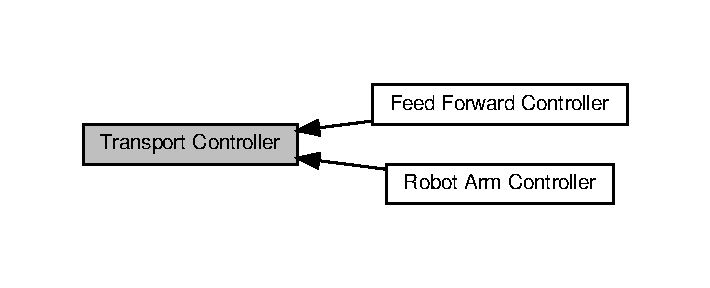
\includegraphics[width=341pt]{d3/d47/group__transport__controller}
\end{center}
\end{figure}
\subsection*{Modules}
\begin{DoxyCompactItemize}
\item 
\hyperlink{group__group__feed__forward}{Feed Forward Controller}
\item 
\hyperlink{group__group__arm__controller}{Robot Arm Controller}
\end{DoxyCompactItemize}
\subsection*{Functions}
\begin{DoxyCompactItemize}
\item 
void \hyperlink{group__transport__controller_ga465b07e16106af072ed5315010fa876c}{convert\+Msg} (Eigen\+::\+Quaterniond \&quat, std\+\_\+msgs\+::\+Float64 \&msg)
\begin{DoxyCompactList}\small\item\em Convert an float64 z-\/axis angle to an eigen quaternion. \end{DoxyCompactList}\item 
void \hyperlink{group__transport__controller_gad42169e0be94216cd31a8a360a848155}{convert\+Msg} (Eigen\+::\+Quaterniond \&quat, geometry\+\_\+msgs\+::\+Transform \&msg)
\begin{DoxyCompactList}\small\item\em Convert Orientation of a Transform geometry message to an eigen quaternion. \end{DoxyCompactList}\item 
void \hyperlink{group__transport__controller_ga34987bf2293cc8aa5fac7ac60e6510ef}{convert\+Msg} (Eigen\+::\+Quaterniond \&quat, geometry\+\_\+msgs\+::\+Transform\+Stamped \&msg)
\begin{DoxyCompactList}\small\item\em Convert an Stamped\+Transform geometry message to an eigen quaternion. \end{DoxyCompactList}\item 
void \hyperlink{group__transport__controller_gadc07db93efb76fd809b67b74dd13b939}{convert\+Msg} (Eigen\+::\+Quaterniond \&quat, geometry\+\_\+msgs\+::\+Pose \&msg)
\begin{DoxyCompactList}\small\item\em Convert an Pose geometry message to an eigen quaternion. \end{DoxyCompactList}\item 
void \hyperlink{group__transport__controller_ga8257db2bb94ec53eadfe87d04b38cc0b}{convert\+Msg} (Eigen\+::\+Quaterniond \&quat, geometry\+\_\+msgs\+::\+Pose\+Stamped \&msg)
\begin{DoxyCompactList}\small\item\em Convert an stamped pose geometry message to an eigen quaternion. \end{DoxyCompactList}\item 
void \hyperlink{group__transport__controller_gafde5764b46f0189c2aea14ed57434708}{convert\+Msg} (Eigen\+::\+Matrix$<$ double, 7, 1 $>$ \&pose, geometry\+\_\+msgs\+::\+Pose \&msg)
\begin{DoxyCompactList}\small\item\em Convert an pose geometry message to an Eigen pose vector (x, y, z, w, x, y, z) \end{DoxyCompactList}\item 
void \hyperlink{group__transport__controller_ga9e842115a5f448ab0e3ba9fea93d5179}{convert\+Msg} (Eigen\+::\+Matrix$<$ double, 7, 1 $>$ \&pose, geometry\+\_\+msgs\+::\+Pose\+Stamped \&msg)
\begin{DoxyCompactList}\small\item\em Convert an stamepd pose geometry message to an Eigen pose vector (x, y, z, w, x, y, z) \end{DoxyCompactList}\item 
void \hyperlink{group__transport__controller_ga7beb50c98e49263d05b3b819be58d76c}{convert\+Msg} (geometry\+\_\+msgs\+::\+Pose \&msg, Eigen\+::\+Matrix$<$ double, 7, 1 $>$ \&pose)
\begin{DoxyCompactList}\small\item\em Convert an Eigen pose vector (x, y, z, w, x, y, z) to a pose geometry message. \end{DoxyCompactList}\item 
void \hyperlink{group__transport__controller_gaf1628de186f2d90b064f8c8b36beef53}{convert\+Msg} (geometry\+\_\+msgs\+::\+Pose\+Stamped \&msg, Eigen\+::\+Matrix$<$ double, 7, 1 $>$ \&pose)
\begin{DoxyCompactList}\small\item\em Convert an Eigen pose vector (x, y, z, w, x, y, z) to a stamepd pose geometry message. \end{DoxyCompactList}\item 
void \hyperlink{group__transport__controller_ga45b2bbef58d2c60ff8eeb77d221f2ab7}{convert\+Msg} (geometry\+\_\+msgs\+::\+Pose \&pose, geometry\+\_\+msgs\+::\+Transform \&transform)
\begin{DoxyCompactList}\small\item\em Convert an Eigen pose vector (x, y, z, w, x, y, z) to a transform geometry message. \end{DoxyCompactList}\item 
void \hyperlink{group__transport__controller_gaf99f4d3d714176ee5a3d235ffabb7d3f}{convert\+Msg} (geometry\+\_\+msgs\+::\+Pose\+Stamped \&pose, geometry\+\_\+msgs\+::\+Transform\+Stamped \&transform\+Stamped)
\begin{DoxyCompactList}\small\item\em Convert a stamped transform geometry message to a stamped pose geometry message. \end{DoxyCompactList}\item 
void \hyperlink{group__transport__controller_ga27bedbf17c4aa6e228239ef1f1009e2b}{convert\+Msg} (geometry\+\_\+msgs\+::\+Transform \&transform, geometry\+\_\+msgs\+::\+Pose \&pose)
\begin{DoxyCompactList}\small\item\em Convert a geometry pos messag to a geometry transfomr message. \end{DoxyCompactList}\item 
void \hyperlink{group__transport__controller_ga83f417b8e164774e4926508549543498}{convert\+Msg} (geometry\+\_\+msgs\+::\+Transform\+Stamped \&transform, geometry\+\_\+msgs\+::\+Pose\+Stamped \&pose)
\begin{DoxyCompactList}\small\item\em Convert a geometry stamped pose message to a stamped transform geometry message. \end{DoxyCompactList}\end{DoxyCompactItemize}


\subsection{Detailed Description}
Module that holds all controllers for transport purpose. 



\subsection{Function Documentation}
\mbox{\Hypertarget{group__transport__controller_ga465b07e16106af072ed5315010fa876c}\label{group__transport__controller_ga465b07e16106af072ed5315010fa876c}} 
\index{Transport Controller@{Transport Controller}!convert\+Msg@{convert\+Msg}}
\index{convert\+Msg@{convert\+Msg}!Transport Controller@{Transport Controller}}
\subsubsection{\texorpdfstring{convert\+Msg()}{convertMsg()}\hspace{0.1cm}{\footnotesize\ttfamily [1/13]}}
{\footnotesize\ttfamily void convert\+Msg (\begin{DoxyParamCaption}\item[{Eigen\+::\+Quaterniond \&}]{quat,  }\item[{std\+\_\+msgs\+::\+Float64 \&}]{msg }\end{DoxyParamCaption})}



Convert an float64 z-\/axis angle to an eigen quaternion. 


\begin{DoxyParams}{Parameters}
{\em msg} & Float64 ros message with z-\/axis angle \\
\hline
{\em quat} & Eigen quaterniond the quaternion is stored in \\
\hline
\end{DoxyParams}
\mbox{\Hypertarget{group__transport__controller_gad42169e0be94216cd31a8a360a848155}\label{group__transport__controller_gad42169e0be94216cd31a8a360a848155}} 
\index{Transport Controller@{Transport Controller}!convert\+Msg@{convert\+Msg}}
\index{convert\+Msg@{convert\+Msg}!Transport Controller@{Transport Controller}}
\subsubsection{\texorpdfstring{convert\+Msg()}{convertMsg()}\hspace{0.1cm}{\footnotesize\ttfamily [2/13]}}
{\footnotesize\ttfamily void convert\+Msg (\begin{DoxyParamCaption}\item[{Eigen\+::\+Quaterniond \&}]{quat,  }\item[{geometry\+\_\+msgs\+::\+Transform \&}]{msg }\end{DoxyParamCaption})}



Convert Orientation of a Transform geometry message to an eigen quaternion. 


\begin{DoxyParams}{Parameters}
{\em msg} & Message that holds the transform \\
\hline
{\em quat} & Quaternion the eigen quaternion is stored in \\
\hline
\end{DoxyParams}
\mbox{\Hypertarget{group__transport__controller_ga34987bf2293cc8aa5fac7ac60e6510ef}\label{group__transport__controller_ga34987bf2293cc8aa5fac7ac60e6510ef}} 
\index{Transport Controller@{Transport Controller}!convert\+Msg@{convert\+Msg}}
\index{convert\+Msg@{convert\+Msg}!Transport Controller@{Transport Controller}}
\subsubsection{\texorpdfstring{convert\+Msg()}{convertMsg()}\hspace{0.1cm}{\footnotesize\ttfamily [3/13]}}
{\footnotesize\ttfamily void convert\+Msg (\begin{DoxyParamCaption}\item[{Eigen\+::\+Quaterniond \&}]{quat,  }\item[{geometry\+\_\+msgs\+::\+Transform\+Stamped \&}]{msg }\end{DoxyParamCaption})}



Convert an Stamped\+Transform geometry message to an eigen quaternion. 


\begin{DoxyParams}{Parameters}
{\em msg} & Message that holds the stamped transform \\
\hline
{\em quat} & Quternion the eigen quaternion is stored in \\
\hline
\end{DoxyParams}
\mbox{\Hypertarget{group__transport__controller_gadc07db93efb76fd809b67b74dd13b939}\label{group__transport__controller_gadc07db93efb76fd809b67b74dd13b939}} 
\index{Transport Controller@{Transport Controller}!convert\+Msg@{convert\+Msg}}
\index{convert\+Msg@{convert\+Msg}!Transport Controller@{Transport Controller}}
\subsubsection{\texorpdfstring{convert\+Msg()}{convertMsg()}\hspace{0.1cm}{\footnotesize\ttfamily [4/13]}}
{\footnotesize\ttfamily void convert\+Msg (\begin{DoxyParamCaption}\item[{Eigen\+::\+Quaterniond \&}]{quat,  }\item[{geometry\+\_\+msgs\+::\+Pose \&}]{msg }\end{DoxyParamCaption})}



Convert an Pose geometry message to an eigen quaternion. 


\begin{DoxyParams}{Parameters}
{\em msg} & Message that holds the pose \\
\hline
{\em quat} & Quternion the eigen quaternion is stored in \\
\hline
\end{DoxyParams}
\mbox{\Hypertarget{group__transport__controller_ga8257db2bb94ec53eadfe87d04b38cc0b}\label{group__transport__controller_ga8257db2bb94ec53eadfe87d04b38cc0b}} 
\index{Transport Controller@{Transport Controller}!convert\+Msg@{convert\+Msg}}
\index{convert\+Msg@{convert\+Msg}!Transport Controller@{Transport Controller}}
\subsubsection{\texorpdfstring{convert\+Msg()}{convertMsg()}\hspace{0.1cm}{\footnotesize\ttfamily [5/13]}}
{\footnotesize\ttfamily void convert\+Msg (\begin{DoxyParamCaption}\item[{Eigen\+::\+Quaterniond \&}]{quat,  }\item[{geometry\+\_\+msgs\+::\+Pose\+Stamped \&}]{msg }\end{DoxyParamCaption})}



Convert an stamped pose geometry message to an eigen quaternion. 


\begin{DoxyParams}{Parameters}
{\em msg} & Message that holds the stamped pose \\
\hline
{\em quat} & Quternion the eigen quaternion is stored in \\
\hline
\end{DoxyParams}
\mbox{\Hypertarget{group__transport__controller_gafde5764b46f0189c2aea14ed57434708}\label{group__transport__controller_gafde5764b46f0189c2aea14ed57434708}} 
\index{Transport Controller@{Transport Controller}!convert\+Msg@{convert\+Msg}}
\index{convert\+Msg@{convert\+Msg}!Transport Controller@{Transport Controller}}
\subsubsection{\texorpdfstring{convert\+Msg()}{convertMsg()}\hspace{0.1cm}{\footnotesize\ttfamily [6/13]}}
{\footnotesize\ttfamily void convert\+Msg (\begin{DoxyParamCaption}\item[{Eigen\+::\+Matrix$<$ double, 7, 1 $>$ \&}]{pose,  }\item[{geometry\+\_\+msgs\+::\+Pose \&}]{msg }\end{DoxyParamCaption})}



Convert an pose geometry message to an Eigen pose vector (x, y, z, w, x, y, z) 


\begin{DoxyParams}{Parameters}
{\em msg} & Message that holds the pose \\
\hline
{\em pose} & Matrix (Vector) the eigen pose vector is stored in \\
\hline
\end{DoxyParams}
\mbox{\Hypertarget{group__transport__controller_ga9e842115a5f448ab0e3ba9fea93d5179}\label{group__transport__controller_ga9e842115a5f448ab0e3ba9fea93d5179}} 
\index{Transport Controller@{Transport Controller}!convert\+Msg@{convert\+Msg}}
\index{convert\+Msg@{convert\+Msg}!Transport Controller@{Transport Controller}}
\subsubsection{\texorpdfstring{convert\+Msg()}{convertMsg()}\hspace{0.1cm}{\footnotesize\ttfamily [7/13]}}
{\footnotesize\ttfamily void convert\+Msg (\begin{DoxyParamCaption}\item[{Eigen\+::\+Matrix$<$ double, 7, 1 $>$ \&}]{pose,  }\item[{geometry\+\_\+msgs\+::\+Pose\+Stamped \&}]{msg }\end{DoxyParamCaption})}



Convert an stamepd pose geometry message to an Eigen pose vector (x, y, z, w, x, y, z) 


\begin{DoxyParams}{Parameters}
{\em msg} & Message that holds the pose \\
\hline
{\em pose} & Matrix (Vector) the eigen pose vector is stored in \\
\hline
\end{DoxyParams}
\mbox{\Hypertarget{group__transport__controller_ga7beb50c98e49263d05b3b819be58d76c}\label{group__transport__controller_ga7beb50c98e49263d05b3b819be58d76c}} 
\index{Transport Controller@{Transport Controller}!convert\+Msg@{convert\+Msg}}
\index{convert\+Msg@{convert\+Msg}!Transport Controller@{Transport Controller}}
\subsubsection{\texorpdfstring{convert\+Msg()}{convertMsg()}\hspace{0.1cm}{\footnotesize\ttfamily [8/13]}}
{\footnotesize\ttfamily void convert\+Msg (\begin{DoxyParamCaption}\item[{geometry\+\_\+msgs\+::\+Pose \&}]{msg,  }\item[{Eigen\+::\+Matrix$<$ double, 7, 1 $>$ \&}]{pose }\end{DoxyParamCaption})}



Convert an Eigen pose vector (x, y, z, w, x, y, z) to a pose geometry message. 


\begin{DoxyParams}{Parameters}
{\em msg} & Message that the pose is stored in \\
\hline
{\em pose} & Matrix (Vector) that holds the pose \\
\hline
\end{DoxyParams}
\mbox{\Hypertarget{group__transport__controller_gaf1628de186f2d90b064f8c8b36beef53}\label{group__transport__controller_gaf1628de186f2d90b064f8c8b36beef53}} 
\index{Transport Controller@{Transport Controller}!convert\+Msg@{convert\+Msg}}
\index{convert\+Msg@{convert\+Msg}!Transport Controller@{Transport Controller}}
\subsubsection{\texorpdfstring{convert\+Msg()}{convertMsg()}\hspace{0.1cm}{\footnotesize\ttfamily [9/13]}}
{\footnotesize\ttfamily void convert\+Msg (\begin{DoxyParamCaption}\item[{geometry\+\_\+msgs\+::\+Pose\+Stamped \&}]{msg,  }\item[{Eigen\+::\+Matrix$<$ double, 7, 1 $>$ \&}]{pose }\end{DoxyParamCaption})}



Convert an Eigen pose vector (x, y, z, w, x, y, z) to a stamepd pose geometry message. 


\begin{DoxyParams}{Parameters}
{\em msg} & Message that the pose is stored in \\
\hline
{\em pose} & Matrix (Vector) that holds the pose \\
\hline
\end{DoxyParams}
\mbox{\Hypertarget{group__transport__controller_ga45b2bbef58d2c60ff8eeb77d221f2ab7}\label{group__transport__controller_ga45b2bbef58d2c60ff8eeb77d221f2ab7}} 
\index{Transport Controller@{Transport Controller}!convert\+Msg@{convert\+Msg}}
\index{convert\+Msg@{convert\+Msg}!Transport Controller@{Transport Controller}}
\subsubsection{\texorpdfstring{convert\+Msg()}{convertMsg()}\hspace{0.1cm}{\footnotesize\ttfamily [10/13]}}
{\footnotesize\ttfamily void convert\+Msg (\begin{DoxyParamCaption}\item[{geometry\+\_\+msgs\+::\+Pose \&}]{pose,  }\item[{geometry\+\_\+msgs\+::\+Transform \&}]{transform }\end{DoxyParamCaption})}



Convert an Eigen pose vector (x, y, z, w, x, y, z) to a transform geometry message. 


\begin{DoxyParams}{Parameters}
{\em msg} & Message that the pose is stored in \\
\hline
{\em pose} & Matrix (Vector) that holds the pose \\
\hline
\end{DoxyParams}
\mbox{\Hypertarget{group__transport__controller_gaf99f4d3d714176ee5a3d235ffabb7d3f}\label{group__transport__controller_gaf99f4d3d714176ee5a3d235ffabb7d3f}} 
\index{Transport Controller@{Transport Controller}!convert\+Msg@{convert\+Msg}}
\index{convert\+Msg@{convert\+Msg}!Transport Controller@{Transport Controller}}
\subsubsection{\texorpdfstring{convert\+Msg()}{convertMsg()}\hspace{0.1cm}{\footnotesize\ttfamily [11/13]}}
{\footnotesize\ttfamily void convert\+Msg (\begin{DoxyParamCaption}\item[{geometry\+\_\+msgs\+::\+Pose\+Stamped \&}]{pose,  }\item[{geometry\+\_\+msgs\+::\+Transform\+Stamped \&}]{transform\+Stamped }\end{DoxyParamCaption})}



Convert a stamped transform geometry message to a stamped pose geometry message. 


\begin{DoxyParams}{Parameters}
{\em pose} & Stamped pose the pose is stored in \\
\hline
{\em transform\+Stamped} & The geometry msgs that holds the transform \\
\hline
\end{DoxyParams}
\mbox{\Hypertarget{group__transport__controller_ga27bedbf17c4aa6e228239ef1f1009e2b}\label{group__transport__controller_ga27bedbf17c4aa6e228239ef1f1009e2b}} 
\index{Transport Controller@{Transport Controller}!convert\+Msg@{convert\+Msg}}
\index{convert\+Msg@{convert\+Msg}!Transport Controller@{Transport Controller}}
\subsubsection{\texorpdfstring{convert\+Msg()}{convertMsg()}\hspace{0.1cm}{\footnotesize\ttfamily [12/13]}}
{\footnotesize\ttfamily void convert\+Msg (\begin{DoxyParamCaption}\item[{geometry\+\_\+msgs\+::\+Transform \&}]{transform,  }\item[{geometry\+\_\+msgs\+::\+Pose \&}]{pose }\end{DoxyParamCaption})}



Convert a geometry pos messag to a geometry transfomr message. 


\begin{DoxyParams}{Parameters}
{\em transform} & Message the transform is stored in \\
\hline
{\em pose} & Message that holds the pose \\
\hline
\end{DoxyParams}
\mbox{\Hypertarget{group__transport__controller_ga83f417b8e164774e4926508549543498}\label{group__transport__controller_ga83f417b8e164774e4926508549543498}} 
\index{Transport Controller@{Transport Controller}!convert\+Msg@{convert\+Msg}}
\index{convert\+Msg@{convert\+Msg}!Transport Controller@{Transport Controller}}
\subsubsection{\texorpdfstring{convert\+Msg()}{convertMsg()}\hspace{0.1cm}{\footnotesize\ttfamily [13/13]}}
{\footnotesize\ttfamily void convert\+Msg (\begin{DoxyParamCaption}\item[{geometry\+\_\+msgs\+::\+Transform\+Stamped \&}]{transform,  }\item[{geometry\+\_\+msgs\+::\+Pose\+Stamped \&}]{pose }\end{DoxyParamCaption})}



Convert a geometry stamped pose message to a stamped transform geometry message. 


\begin{DoxyParams}{Parameters}
{\em transform} & Message the stamped transform is stored in \\
\hline
{\em pose} & Message that holds the pose \\
\hline
\end{DoxyParams}

\hypertarget{group__group__feed__forward}{}\section{Feed Forward Controller}
\label{group__group__feed__forward}\index{Feed Forward Controller@{Feed Forward Controller}}
Collaboration diagram for Feed Forward Controller\+:\nopagebreak
\begin{figure}[H]
\begin{center}
\leavevmode
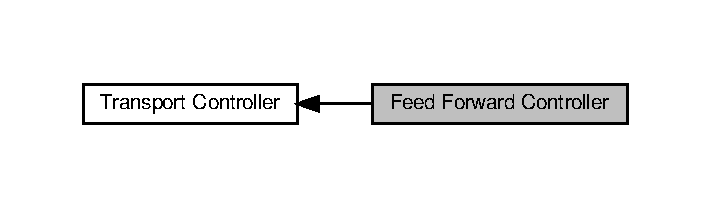
\includegraphics[width=341pt]{db/da6/group__group__feed__forward}
\end{center}
\end{figure}
\subsection*{Classes}
\begin{DoxyCompactItemize}
\item 
class \hyperlink{classOrientationFeedForward}{Orientation\+Feed\+Forward}
\begin{DoxyCompactList}\small\item\em A Orientation feed forward class. It uses a given orientation and calculates a robot arm pose that compansates the motion by the change of orientation (null space motion). \end{DoxyCompactList}\item 
class \hyperlink{classRosOrientationFeedForward}{Ros\+Orientation\+Feed\+Forward$<$ T $>$}
\begin{DoxyCompactList}\small\item\em A Ros implementation of the Orientation\+Feeed\+Forward class. It contains a ros Subscriber that listens to a specific message and uses the message data as input data for the feed forward control. \end{DoxyCompactList}\end{DoxyCompactItemize}


\subsection{Detailed Description}

\hypertarget{group__group__arm__controller}{}\section{Robot Arm Controller}
\label{group__group__arm__controller}\index{Robot Arm Controller@{Robot Arm Controller}}
Collaboration diagram for Robot Arm Controller\+:\nopagebreak
\begin{figure}[H]
\begin{center}
\leavevmode
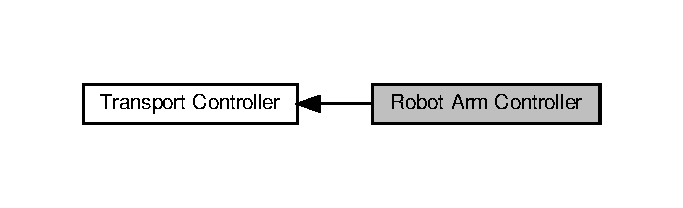
\includegraphics[width=328pt]{d3/d63/group__group__arm__controller}
\end{center}
\end{figure}

\chapter{Class Documentation}
\hypertarget{classOrientationFeedForward}{}\section{Orientation\+Feed\+Forward Class Reference}
\label{classOrientationFeedForward}\index{Orientation\+Feed\+Forward@{Orientation\+Feed\+Forward}}


A Orientation feed forward class. It uses a given orientation and calculates a robot arm pose that compansates the motion by the change of orientation (null space motion).  




{\ttfamily \#include $<$orientation\+\_\+feed\+\_\+forward.\+h$>$}



Inheritance diagram for Orientation\+Feed\+Forward\+:\nopagebreak
\begin{figure}[H]
\begin{center}
\leavevmode
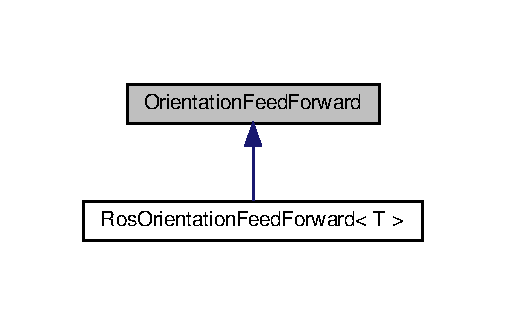
\includegraphics[width=350pt]{dd/d46/classOrientationFeedForward__inherit__graph}
\end{center}
\end{figure}
\subsection*{Public Types}
\begin{DoxyCompactItemize}
\item 
\mbox{\Hypertarget{classOrientationFeedForward_a45f6220dd29a9df06f62eeed86189101}\label{classOrientationFeedForward_a45f6220dd29a9df06f62eeed86189101}} 
typedef Eigen\+::\+Matrix$<$ double, 3, 1 $>$ {\bfseries Position}
\item 
\mbox{\Hypertarget{classOrientationFeedForward_a329654d4c6d79679903a76c624330f99}\label{classOrientationFeedForward_a329654d4c6d79679903a76c624330f99}} 
typedef Eigen\+::\+Quaterniond {\bfseries Orientation}
\item 
\mbox{\Hypertarget{classOrientationFeedForward_a68247ebc7099747e21cbd56d4dbc405a}\label{classOrientationFeedForward_a68247ebc7099747e21cbd56d4dbc405a}} 
typedef Eigen\+::\+Matrix$<$ double, 7, 1 $>$ {\bfseries Pose}
\end{DoxyCompactItemize}
\subsection*{Public Member Functions}
\begin{DoxyCompactItemize}
\item 
\mbox{\Hypertarget{classOrientationFeedForward_aad82bda1b9fa824e321a6c8afad84973}\label{classOrientationFeedForward_aad82bda1b9fa824e321a6c8afad84973}} 
\hyperlink{classOrientationFeedForward_aad82bda1b9fa824e321a6c8afad84973}{Orientation\+Feed\+Forward} ()
\begin{DoxyCompactList}\small\item\em Construct a new Orientation Feed Forward object. \end{DoxyCompactList}\item 
\hyperlink{classOrientationFeedForward_a0ae1aba3b3e0abf84828a9db008b6f69}{Orientation\+Feed\+Forward} (Position pos\+\_\+offf, Orientation ori\+\_\+off)
\begin{DoxyCompactList}\small\item\em Construct a new Orientation Feed Forward object. \end{DoxyCompactList}\item 
void \hyperlink{classOrientationFeedForward_aa7d8913f8f9d90e913b478d9adc5ff20}{update\+Orientation} (double angle)
\begin{DoxyCompactList}\small\item\em Updates the current Orientation of the mobile base that has to be feed forwarded. \end{DoxyCompactList}\item 
void \hyperlink{classOrientationFeedForward_aed8f826976135c0cd55408a652993828}{update\+Orientation} (Orientation ori)
\begin{DoxyCompactList}\small\item\em Updates the current Orientation of the mobile base that has to be feed forwarded. \end{DoxyCompactList}\item 
Pose \hyperlink{classOrientationFeedForward_ad31fce2cdf39cbf375457b9aa7ca2219}{get\+Pose} ()
\begin{DoxyCompactList}\small\item\em Get the Pose object for motion control. \end{DoxyCompactList}\item 
void \hyperlink{classOrientationFeedForward_adc105d9a1fe00d6a79fcf38447202709}{set\+Offset} (Position pos\+\_\+off, Orientation ori\+\_\+off)
\begin{DoxyCompactList}\small\item\em Set the Offset object. \end{DoxyCompactList}\item 
void \hyperlink{classOrientationFeedForward_adbd1691b1e930752818624d065acbf1c}{set\+Offset} (Pose pose)
\begin{DoxyCompactList}\small\item\em Set the Offset object. \end{DoxyCompactList}\item 
void \hyperlink{classOrientationFeedForward_a5f69dfd449972707d2ccd07e20fd2c5b}{set\+Desired\+Pose} (Pose pose)
\begin{DoxyCompactList}\small\item\em Set the Desired Pose that has to be hold in mobile base frame. \end{DoxyCompactList}\item 
void \hyperlink{classOrientationFeedForward_ad419aebf0df88282ca6c1dc24adbadb2}{set\+Desired\+Pose} (Position position, Orientation orientation)
\begin{DoxyCompactList}\small\item\em Set the Desired Pose object. \end{DoxyCompactList}\end{DoxyCompactItemize}


\subsection{Constructor \& Destructor Documentation}
\mbox{\Hypertarget{classOrientationFeedForward_a0ae1aba3b3e0abf84828a9db008b6f69}\label{classOrientationFeedForward_a0ae1aba3b3e0abf84828a9db008b6f69}} 
\index{Orientation\+Feed\+Forward@{Orientation\+Feed\+Forward}!Orientation\+Feed\+Forward@{Orientation\+Feed\+Forward}}
\index{Orientation\+Feed\+Forward@{Orientation\+Feed\+Forward}!Orientation\+Feed\+Forward@{Orientation\+Feed\+Forward}}
\subsubsection{\texorpdfstring{Orientation\+Feed\+Forward()}{OrientationFeedForward()}}
{\footnotesize\ttfamily Orientation\+Feed\+Forward\+::\+Orientation\+Feed\+Forward (\begin{DoxyParamCaption}\item[{Position}]{pos\+\_\+offf,  }\item[{Orientation}]{ori\+\_\+off }\end{DoxyParamCaption})}


\begin{DoxyParams}{Parameters}
{\em ori\+\_\+off} & The Orientation offset the Robot base has with respect to the mobile base frame \\
\hline
{\em pos\+\_\+offf} & The Position offset the Robot base has with respect to the mobile base frame \\
\hline
\end{DoxyParams}


\subsection{Member Function Documentation}
\mbox{\Hypertarget{classOrientationFeedForward_ad31fce2cdf39cbf375457b9aa7ca2219}\label{classOrientationFeedForward_ad31fce2cdf39cbf375457b9aa7ca2219}} 
\index{Orientation\+Feed\+Forward@{Orientation\+Feed\+Forward}!get\+Pose@{get\+Pose}}
\index{get\+Pose@{get\+Pose}!Orientation\+Feed\+Forward@{Orientation\+Feed\+Forward}}
\subsubsection{\texorpdfstring{get\+Pose()}{getPose()}}
{\footnotesize\ttfamily Orientation\+Feed\+Forward\+::\+Pose Orientation\+Feed\+Forward\+::get\+Pose (\begin{DoxyParamCaption}{ }\end{DoxyParamCaption})}

\begin{DoxyReturn}{Returns}
Pose in robot base frame wich can be forwarded to the robot motion control 
\end{DoxyReturn}
\mbox{\Hypertarget{classOrientationFeedForward_a5f69dfd449972707d2ccd07e20fd2c5b}\label{classOrientationFeedForward_a5f69dfd449972707d2ccd07e20fd2c5b}} 
\index{Orientation\+Feed\+Forward@{Orientation\+Feed\+Forward}!set\+Desired\+Pose@{set\+Desired\+Pose}}
\index{set\+Desired\+Pose@{set\+Desired\+Pose}!Orientation\+Feed\+Forward@{Orientation\+Feed\+Forward}}
\subsubsection{\texorpdfstring{set\+Desired\+Pose()}{setDesiredPose()}\hspace{0.1cm}{\footnotesize\ttfamily [1/2]}}
{\footnotesize\ttfamily void Orientation\+Feed\+Forward\+::set\+Desired\+Pose (\begin{DoxyParamCaption}\item[{Pose}]{pose }\end{DoxyParamCaption})}


\begin{DoxyParams}{Parameters}
{\em pose} & Desired Pose with in mobile base frame \\
\hline
\end{DoxyParams}
\mbox{\Hypertarget{classOrientationFeedForward_ad419aebf0df88282ca6c1dc24adbadb2}\label{classOrientationFeedForward_ad419aebf0df88282ca6c1dc24adbadb2}} 
\index{Orientation\+Feed\+Forward@{Orientation\+Feed\+Forward}!set\+Desired\+Pose@{set\+Desired\+Pose}}
\index{set\+Desired\+Pose@{set\+Desired\+Pose}!Orientation\+Feed\+Forward@{Orientation\+Feed\+Forward}}
\subsubsection{\texorpdfstring{set\+Desired\+Pose()}{setDesiredPose()}\hspace{0.1cm}{\footnotesize\ttfamily [2/2]}}
{\footnotesize\ttfamily void Orientation\+Feed\+Forward\+::set\+Desired\+Pose (\begin{DoxyParamCaption}\item[{Position}]{position,  }\item[{Orientation}]{orientation }\end{DoxyParamCaption})}


\begin{DoxyParams}{Parameters}
{\em position} & Position that has to be hold by the endeffektor defined in mobile base frame \\
\hline
{\em orientation} & Orientation that has to be hold by the endeffektor defined in robot base frame \\
\hline
\end{DoxyParams}
\mbox{\Hypertarget{classOrientationFeedForward_adc105d9a1fe00d6a79fcf38447202709}\label{classOrientationFeedForward_adc105d9a1fe00d6a79fcf38447202709}} 
\index{Orientation\+Feed\+Forward@{Orientation\+Feed\+Forward}!set\+Offset@{set\+Offset}}
\index{set\+Offset@{set\+Offset}!Orientation\+Feed\+Forward@{Orientation\+Feed\+Forward}}
\subsubsection{\texorpdfstring{set\+Offset()}{setOffset()}\hspace{0.1cm}{\footnotesize\ttfamily [1/2]}}
{\footnotesize\ttfamily void Orientation\+Feed\+Forward\+::set\+Offset (\begin{DoxyParamCaption}\item[{Position}]{pos\+\_\+off,  }\item[{Orientation}]{ori\+\_\+off }\end{DoxyParamCaption})}


\begin{DoxyParams}{Parameters}
{\em ori\+\_\+off} & Orientation of the Offset (from the mobile base frame and the robot frame) \\
\hline
{\em pos\+\_\+off} & Position of the Offset (from mobile base frame and the robot frame) \\
\hline
\end{DoxyParams}
\mbox{\Hypertarget{classOrientationFeedForward_adbd1691b1e930752818624d065acbf1c}\label{classOrientationFeedForward_adbd1691b1e930752818624d065acbf1c}} 
\index{Orientation\+Feed\+Forward@{Orientation\+Feed\+Forward}!set\+Offset@{set\+Offset}}
\index{set\+Offset@{set\+Offset}!Orientation\+Feed\+Forward@{Orientation\+Feed\+Forward}}
\subsubsection{\texorpdfstring{set\+Offset()}{setOffset()}\hspace{0.1cm}{\footnotesize\ttfamily [2/2]}}
{\footnotesize\ttfamily void Orientation\+Feed\+Forward\+::set\+Offset (\begin{DoxyParamCaption}\item[{Pose}]{pose }\end{DoxyParamCaption})}


\begin{DoxyParams}{Parameters}
{\em ori\+\_\+off} & Orientation of the Offset (from the mobile base frame and the robot frame) \\
\hline
{\em pos\+\_\+off} & Position of the Offset (from mobile base frame and the robot frame) \\
\hline
\end{DoxyParams}
\mbox{\Hypertarget{classOrientationFeedForward_aa7d8913f8f9d90e913b478d9adc5ff20}\label{classOrientationFeedForward_aa7d8913f8f9d90e913b478d9adc5ff20}} 
\index{Orientation\+Feed\+Forward@{Orientation\+Feed\+Forward}!update\+Orientation@{update\+Orientation}}
\index{update\+Orientation@{update\+Orientation}!Orientation\+Feed\+Forward@{Orientation\+Feed\+Forward}}
\subsubsection{\texorpdfstring{update\+Orientation()}{updateOrientation()}\hspace{0.1cm}{\footnotesize\ttfamily [1/2]}}
{\footnotesize\ttfamily void Orientation\+Feed\+Forward\+::update\+Orientation (\begin{DoxyParamCaption}\item[{double}]{angle }\end{DoxyParamCaption})}


\begin{DoxyParams}{Parameters}
{\em angle} & Angle of the Rotation around z-\/axis \\
\hline
\end{DoxyParams}
\mbox{\Hypertarget{classOrientationFeedForward_aed8f826976135c0cd55408a652993828}\label{classOrientationFeedForward_aed8f826976135c0cd55408a652993828}} 
\index{Orientation\+Feed\+Forward@{Orientation\+Feed\+Forward}!update\+Orientation@{update\+Orientation}}
\index{update\+Orientation@{update\+Orientation}!Orientation\+Feed\+Forward@{Orientation\+Feed\+Forward}}
\subsubsection{\texorpdfstring{update\+Orientation()}{updateOrientation()}\hspace{0.1cm}{\footnotesize\ttfamily [2/2]}}
{\footnotesize\ttfamily void Orientation\+Feed\+Forward\+::update\+Orientation (\begin{DoxyParamCaption}\item[{Orientation}]{ori }\end{DoxyParamCaption})}


\begin{DoxyParams}{Parameters}
{\em ori} & Quaternion of the current Orientation \\
\hline
\end{DoxyParams}


The documentation for this class was generated from the following files\+:\begin{DoxyCompactItemize}
\item 
include/multi\+\_\+robot\+\_\+controller/feed\+\_\+forward/orientation\+\_\+feed\+\_\+forward.\+h\item 
src/feed\+\_\+forward/orientation\+\_\+feed\+\_\+forward.\+cpp\end{DoxyCompactItemize}

\hypertarget{classRosOrientationFeedForward}{}\section{Ros\+Orientation\+Feed\+Forward$<$ T $>$ Class Template Reference}
\label{classRosOrientationFeedForward}\index{Ros\+Orientation\+Feed\+Forward$<$ T $>$@{Ros\+Orientation\+Feed\+Forward$<$ T $>$}}


A Ros implementation of the Orientation\+Feeed\+Forward class. It contains a ros Subscriber that listens to a specific message and uses the message data as input data for the feed forward control.  




{\ttfamily \#include $<$ros\+\_\+orientation\+\_\+feed\+\_\+forward.\+h$>$}



Inheritance diagram for Ros\+Orientation\+Feed\+Forward$<$ T $>$\+:\nopagebreak
\begin{figure}[H]
\begin{center}
\leavevmode
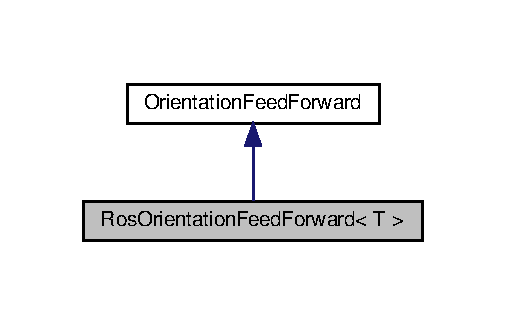
\includegraphics[width=243pt]{d6/d61/classRosOrientationFeedForward__inherit__graph}
\end{center}
\end{figure}


Collaboration diagram for Ros\+Orientation\+Feed\+Forward$<$ T $>$\+:\nopagebreak
\begin{figure}[H]
\begin{center}
\leavevmode
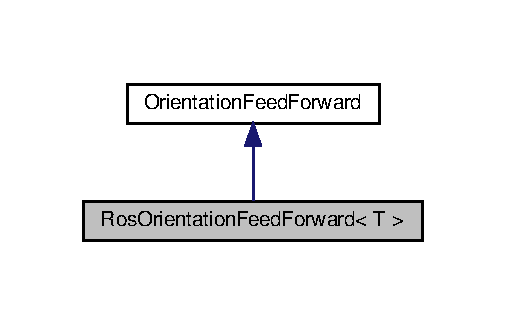
\includegraphics[width=243pt]{df/d60/classRosOrientationFeedForward__coll__graph}
\end{center}
\end{figure}
\subsection*{Public Member Functions}
\begin{DoxyCompactItemize}
\item 
\hyperlink{classRosOrientationFeedForward_acf445e9c7d9be8a85ac899c0d6f7387b}{Ros\+Orientation\+Feed\+Forward} (ros\+::\+Node\+Handle \&nh, std\+::string topic)
\begin{DoxyCompactList}\small\item\em Construct a new Ros Orientation Feed Forward object. \end{DoxyCompactList}\end{DoxyCompactItemize}
\subsection*{Additional Inherited Members}


\subsection{Detailed Description}
\subsubsection*{template$<$class T$>$\newline
class Ros\+Orientation\+Feed\+Forward$<$ T $>$}

A Ros implementation of the Orientation\+Feeed\+Forward class. It contains a ros Subscriber that listens to a specific message and uses the message data as input data for the feed forward control. 


\begin{DoxyTemplParams}{Template Parameters}
{\em T} & Message type the subcriber is listeneing to. A convert\+Msg fucntion has to be implemented for it. \\
\hline
\end{DoxyTemplParams}


\subsection{Constructor \& Destructor Documentation}
\mbox{\Hypertarget{classRosOrientationFeedForward_acf445e9c7d9be8a85ac899c0d6f7387b}\label{classRosOrientationFeedForward_acf445e9c7d9be8a85ac899c0d6f7387b}} 
\index{Ros\+Orientation\+Feed\+Forward@{Ros\+Orientation\+Feed\+Forward}!Ros\+Orientation\+Feed\+Forward@{Ros\+Orientation\+Feed\+Forward}}
\index{Ros\+Orientation\+Feed\+Forward@{Ros\+Orientation\+Feed\+Forward}!Ros\+Orientation\+Feed\+Forward@{Ros\+Orientation\+Feed\+Forward}}
\subsubsection{\texorpdfstring{Ros\+Orientation\+Feed\+Forward()}{RosOrientationFeedForward()}}
{\footnotesize\ttfamily template$<$class T $>$ \\
\hyperlink{classRosOrientationFeedForward}{Ros\+Orientation\+Feed\+Forward}$<$ T $>$\+::\hyperlink{classRosOrientationFeedForward}{Ros\+Orientation\+Feed\+Forward} (\begin{DoxyParamCaption}\item[{ros\+::\+Node\+Handle \&}]{nh,  }\item[{std\+::string}]{topic }\end{DoxyParamCaption})}



Construct a new Ros Orientation Feed Forward object. 


\begin{DoxyParams}{Parameters}
{\em nh} & Nodehandle for namespace handling \\
\hline
{\em topic} & Topic name that should be used as input source \\
\hline
\end{DoxyParams}


The documentation for this class was generated from the following files\+:\begin{DoxyCompactItemize}
\item 
include/miranda\+\_\+transport\+\_\+controller/ros\+\_\+orientation\+\_\+feed\+\_\+forward.\+h\item 
src/ros\+\_\+orientation\+\_\+feed\+\_\+forward.\+cpp\end{DoxyCompactItemize}

\chapter{File Documentation}
\hypertarget{msg__conversion_8hpp}{}\section{include/multi\+\_\+robot\+\_\+controller/feed\+\_\+forward/msg\+\_\+conversion.hpp File Reference}
\label{msg__conversion_8hpp}\index{include/multi\+\_\+robot\+\_\+controller/feed\+\_\+forward/msg\+\_\+conversion.\+hpp@{include/multi\+\_\+robot\+\_\+controller/feed\+\_\+forward/msg\+\_\+conversion.\+hpp}}
{\ttfamily \#include $<$eigen3/\+Eigen/\+Dense$>$}\newline
{\ttfamily \#include $<$geometry\+\_\+msgs/\+Transform\+Stamped.\+h$>$}\newline
{\ttfamily \#include $<$geometry\+\_\+msgs/\+Transform.\+h$>$}\newline
{\ttfamily \#include $<$geometry\+\_\+msgs/\+Pose\+Stamped.\+h$>$}\newline
{\ttfamily \#include $<$geometry\+\_\+msgs/\+Pose.\+h$>$}\newline
{\ttfamily \#include $<$std\+\_\+msgs/\+Float64.\+h$>$}\newline
Include dependency graph for msg\+\_\+conversion.\+hpp\+:\nopagebreak
\begin{figure}[H]
\begin{center}
\leavevmode
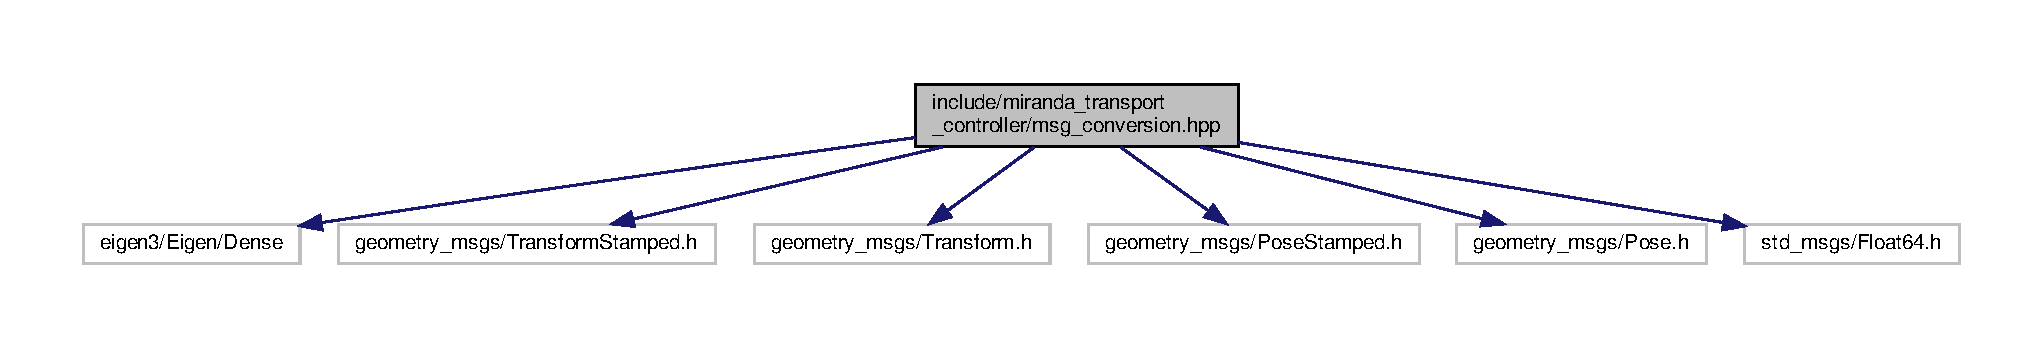
\includegraphics[width=350pt]{d9/d5a/msg__conversion_8hpp__incl}
\end{center}
\end{figure}
This graph shows which files directly or indirectly include this file\+:\nopagebreak
\begin{figure}[H]
\begin{center}
\leavevmode
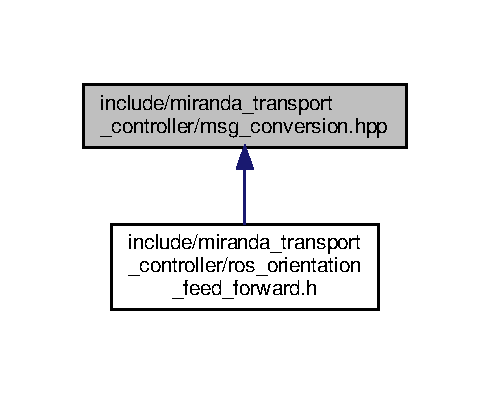
\includegraphics[width=350pt]{de/d06/msg__conversion_8hpp__dep__incl}
\end{center}
\end{figure}
\subsection*{Functions}
\begin{DoxyCompactItemize}
\item 
void \hyperlink{group__MultiRobotController_ga465b07e16106af072ed5315010fa876c}{convert\+Msg} (Eigen\+::\+Quaterniond \&quat, std\+\_\+msgs\+::\+Float64 \&msg)
\begin{DoxyCompactList}\small\item\em Convert an float64 z-\/axis angle to an eigen quaternion. \end{DoxyCompactList}\item 
void \hyperlink{group__MultiRobotController_gad42169e0be94216cd31a8a360a848155}{convert\+Msg} (Eigen\+::\+Quaterniond \&quat, geometry\+\_\+msgs\+::\+Transform \&msg)
\begin{DoxyCompactList}\small\item\em Convert Orientation of a Transform geometry message to an eigen quaternion. \end{DoxyCompactList}\item 
void \hyperlink{group__MultiRobotController_ga34987bf2293cc8aa5fac7ac60e6510ef}{convert\+Msg} (Eigen\+::\+Quaterniond \&quat, geometry\+\_\+msgs\+::\+Transform\+Stamped \&msg)
\begin{DoxyCompactList}\small\item\em Convert an Stamped\+Transform geometry message to an eigen quaternion. \end{DoxyCompactList}\item 
void \hyperlink{group__MultiRobotController_gadc07db93efb76fd809b67b74dd13b939}{convert\+Msg} (Eigen\+::\+Quaterniond \&quat, geometry\+\_\+msgs\+::\+Pose \&msg)
\begin{DoxyCompactList}\small\item\em Convert an Pose geometry message to an eigen quaternion. \end{DoxyCompactList}\item 
void \hyperlink{group__MultiRobotController_ga8257db2bb94ec53eadfe87d04b38cc0b}{convert\+Msg} (Eigen\+::\+Quaterniond \&quat, geometry\+\_\+msgs\+::\+Pose\+Stamped \&msg)
\begin{DoxyCompactList}\small\item\em Convert an stamped pose geometry message to an eigen quaternion. \end{DoxyCompactList}\item 
void \hyperlink{group__MultiRobotController_gafde5764b46f0189c2aea14ed57434708}{convert\+Msg} (Eigen\+::\+Matrix$<$ double, 7, 1 $>$ \&pose, geometry\+\_\+msgs\+::\+Pose \&msg)
\begin{DoxyCompactList}\small\item\em Convert an pose geometry message to an Eigen pose vector (x, y, z, w, x, y, z) \end{DoxyCompactList}\item 
void \hyperlink{group__MultiRobotController_ga9e842115a5f448ab0e3ba9fea93d5179}{convert\+Msg} (Eigen\+::\+Matrix$<$ double, 7, 1 $>$ \&pose, geometry\+\_\+msgs\+::\+Pose\+Stamped \&msg)
\begin{DoxyCompactList}\small\item\em Convert an stamepd pose geometry message to an Eigen pose vector (x, y, z, w, x, y, z) \end{DoxyCompactList}\item 
void \hyperlink{group__MultiRobotController_ga7beb50c98e49263d05b3b819be58d76c}{convert\+Msg} (geometry\+\_\+msgs\+::\+Pose \&msg, Eigen\+::\+Matrix$<$ double, 7, 1 $>$ \&pose)
\begin{DoxyCompactList}\small\item\em Convert an Eigen pose vector (x, y, z, w, x, y, z) to a pose geometry message. \end{DoxyCompactList}\item 
void \hyperlink{group__MultiRobotController_gaf1628de186f2d90b064f8c8b36beef53}{convert\+Msg} (geometry\+\_\+msgs\+::\+Pose\+Stamped \&msg, Eigen\+::\+Matrix$<$ double, 7, 1 $>$ \&pose)
\begin{DoxyCompactList}\small\item\em Convert an Eigen pose vector (x, y, z, w, x, y, z) to a stamepd pose geometry message. \end{DoxyCompactList}\item 
void \hyperlink{group__MultiRobotController_ga45b2bbef58d2c60ff8eeb77d221f2ab7}{convert\+Msg} (geometry\+\_\+msgs\+::\+Pose \&pose, geometry\+\_\+msgs\+::\+Transform \&transform)
\begin{DoxyCompactList}\small\item\em Convert an Eigen pose vector (x, y, z, w, x, y, z) to a transform geometry message. \end{DoxyCompactList}\item 
void \hyperlink{group__MultiRobotController_gaf99f4d3d714176ee5a3d235ffabb7d3f}{convert\+Msg} (geometry\+\_\+msgs\+::\+Pose\+Stamped \&pose, geometry\+\_\+msgs\+::\+Transform\+Stamped \&transform\+Stamped)
\begin{DoxyCompactList}\small\item\em Convert a stamped transform geometry message to a stamped pose geometry message. \end{DoxyCompactList}\item 
void \hyperlink{group__MultiRobotController_ga21e894dfe1e1216355db06776a630b09}{convert\+Msg} (Eigen\+::\+Matrix$<$ double, 7, 1 $>$ \&pose, geometry\+\_\+msgs\+::\+Transform\+Stamped \&transform\+Stamped)
\begin{DoxyCompactList}\small\item\em Convert a stamped transform geometry message to a eigen pose vector. \end{DoxyCompactList}\item 
void \hyperlink{group__MultiRobotController_ga27bedbf17c4aa6e228239ef1f1009e2b}{convert\+Msg} (geometry\+\_\+msgs\+::\+Transform \&transform, geometry\+\_\+msgs\+::\+Pose \&pose)
\begin{DoxyCompactList}\small\item\em Convert a geometry pos messag to a geometry transfomr message. \end{DoxyCompactList}\item 
void \hyperlink{group__MultiRobotController_ga83f417b8e164774e4926508549543498}{convert\+Msg} (geometry\+\_\+msgs\+::\+Transform\+Stamped \&transform, geometry\+\_\+msgs\+::\+Pose\+Stamped \&pose)
\begin{DoxyCompactList}\small\item\em Convert a geometry stamped pose message to a stamped transform geometry message. \end{DoxyCompactList}\end{DoxyCompactItemize}

%--- End generated contents ---

% Index
\backmatter
\newpage
\phantomsection
\clearemptydoublepage
\addcontentsline{toc}{chapter}{Index}
\printindex

\end{document}
